Another important class of processes at $e^+e^-$ colliders is fermion-antifermion production, which is highly sensitive to various new physics models, as discussed in Sec.~\ref{subsec:phys_ff}. Thereby, the important observables are the polarised total cross sections, in particular in form of the left-right asymmetry $A_{LR}$, as well as the differential cross section as a function of the polar angle, $d\sigma/d \cos{\theta}$, which contains even more information than the forward-backward asymetry $A_{FB}$.

\subsubsection{General experimental aspects}

At center-of-mass energies above the $Z$ pole, di-fermion production will be accompanied frequently by a significant amounts of ISR. E.g.\ at $\sqrt{s}=$250\,GeV, about half of the di-fermion events return to the $Z$ pole. The ISR photons either escape undetected through the beam pipe, or they can be produced under a sufficiently large angle to be measured in the detector {\color{red} [insert ref to detector section for calorimeter acceptance]}.

In the latter case, energy and momentum constraints can be employed to reconstruct the full event kinematics from the angles of the fermions and the photon, {\em without relying on their measured energies or momenta}. This technique offers an excellent opportunity to cross calibrate the energy scales of various subsystems, e.g.\ to calibrate the photon energy scale against the momentum scale of the tracking systems in $e^+e^- \to \mu^+\mu^-\gamma $ events. While in principle also the beam energy spectrum can be obtained from this method, it suffers from large event-by-event statistical fluctuations due to the relatively large width of the $Z$ resonance~\cite{Wilson:2016hne}.

But also in the case that there is no photon detected, the amount of collinear beamstrahlung or ISR energy can be reconstructed from kinematic constraints on an event-by-event basis. In this case, however, the measured momenta of the fermions have to be used. The previously mentioned case of $e^+e^- \to \mu^+\mu^-\gamma $, then provides an excellent method for an in-situ determination of the beam energy spectrum, since the muon momentum scale can be calibrated to 10\,ppm from $J/\psi \to \mu^+\mu^-$ decays~\cite{Wilson:2016hne}.

In presence of beam polarisation, another important observable becomes accessible, namely the left-right asymmetry of 2-fermion processes:
\begin{equation}
A_{LR} = \frac{\sigma_{LR}-\sigma{RL}}{\sigma_{LR}+\sigma{RL}}
\end{equation}
Therby, $\sigma_{LR}$ etc are the chiral cross sections for fully polarised beams, where the first index gives the chirality of the electron and the second index the chirality of the positron.
The cross section for partially polarised beams is calculated from the chiral cross section 

\begin{itemize}
\item Blondel scheme vs global fit
\item role of positron polarisation
\end{itemize}

\subsubsection{$e^+e^- \to e^+ e^- / \mu^+ \mu^- / \tau^+\tau^-$}
\begin{itemize}
\item ILD 250\,GeV LCWS 2017 proceedings~\cite{Yamashiro:2018ant} and talk LCWS 2018
\item SiD 250\,GeV talk LCWS 2018
\item $\tau^+\tau^-$  Taikan LoI~\cite{Suehara:2009nj} and Hieu thesis?
\end{itemize}

\subsubsection{$e^+e^- \to b\bar{b}$}
\begin{itemize}
\item special difficulty: $b$ vs $\bar{b}$ jet identification (jet/vertex charge, Kaon charge, $dE/dx$ plot, role of VTX and TPC)
\item Sviatoslav's results
\end{itemize}

ILD has studied the channel $e^+e^- \to b\bar{b}$ in full, geant4-based detector simulation based on the DBD

\begin{figure*}
       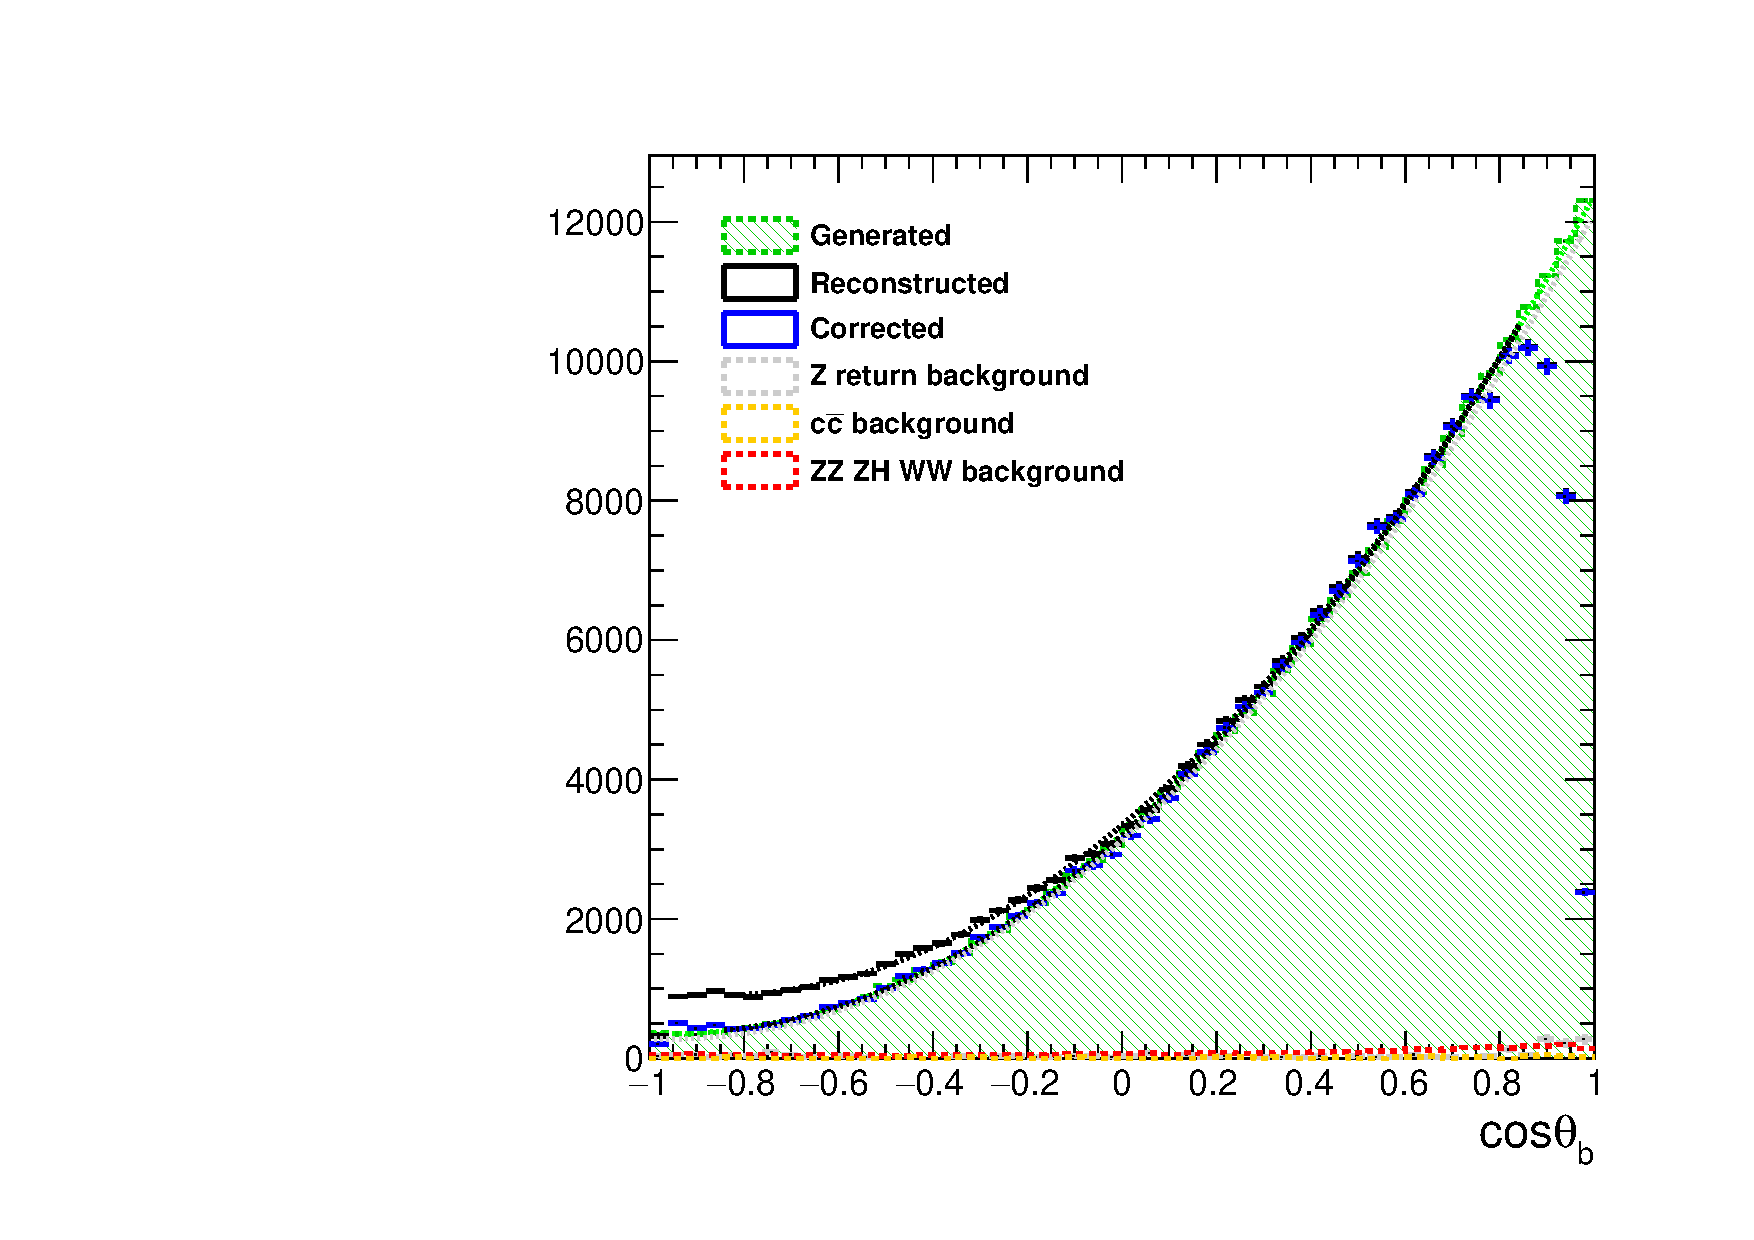
\includegraphics[width=0.45\linewidth]{./chapters/figures/basymmetry-final-left.pdf}
       \llap{\shortstack{%
                       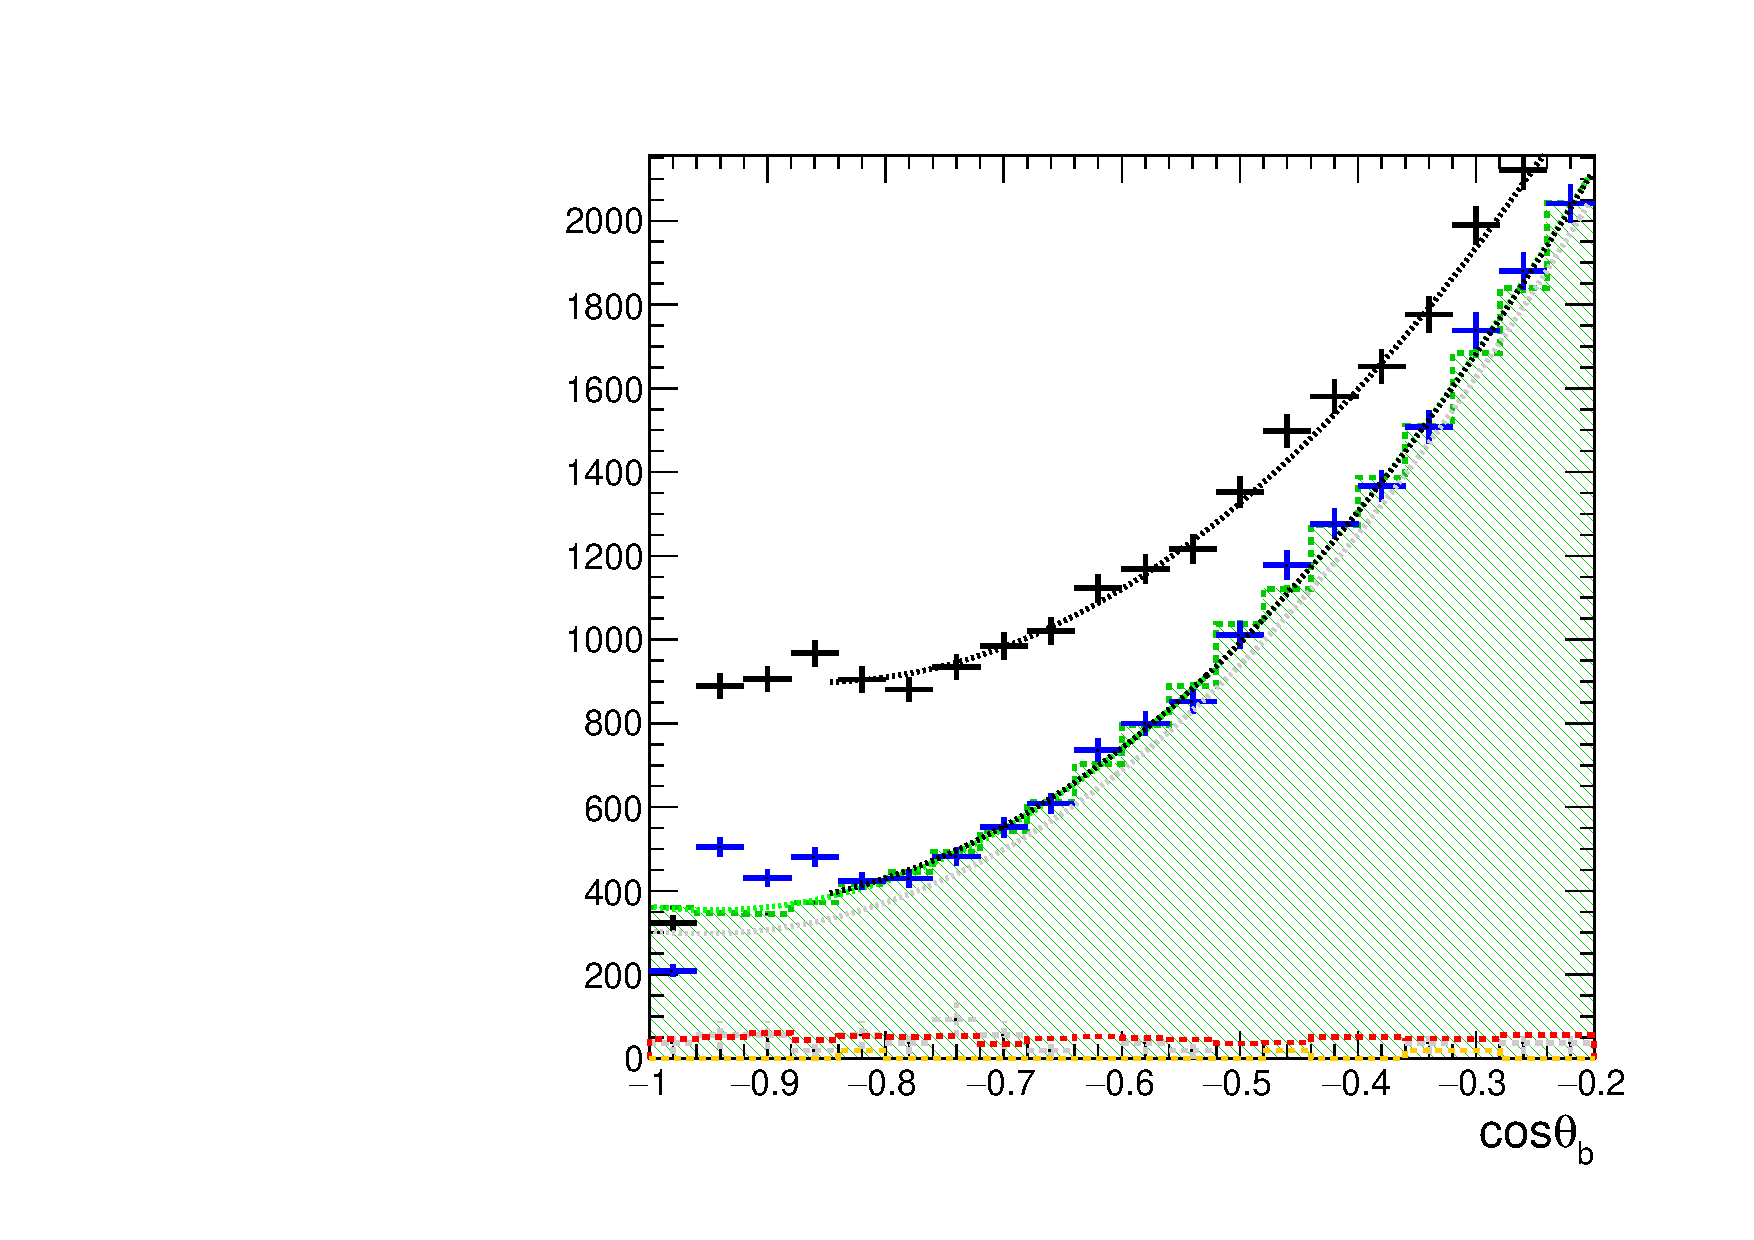
\includegraphics[clip, trim=0cm 0cm 1.8cm 1.7cm, scale=.15]{./chapters/figures/zoom-final.pdf}\\
                       \rule{0ex}{0.67in}%
               }
               \rule{2.2in}{0ex}}
        \hspace{0.2cm}       
        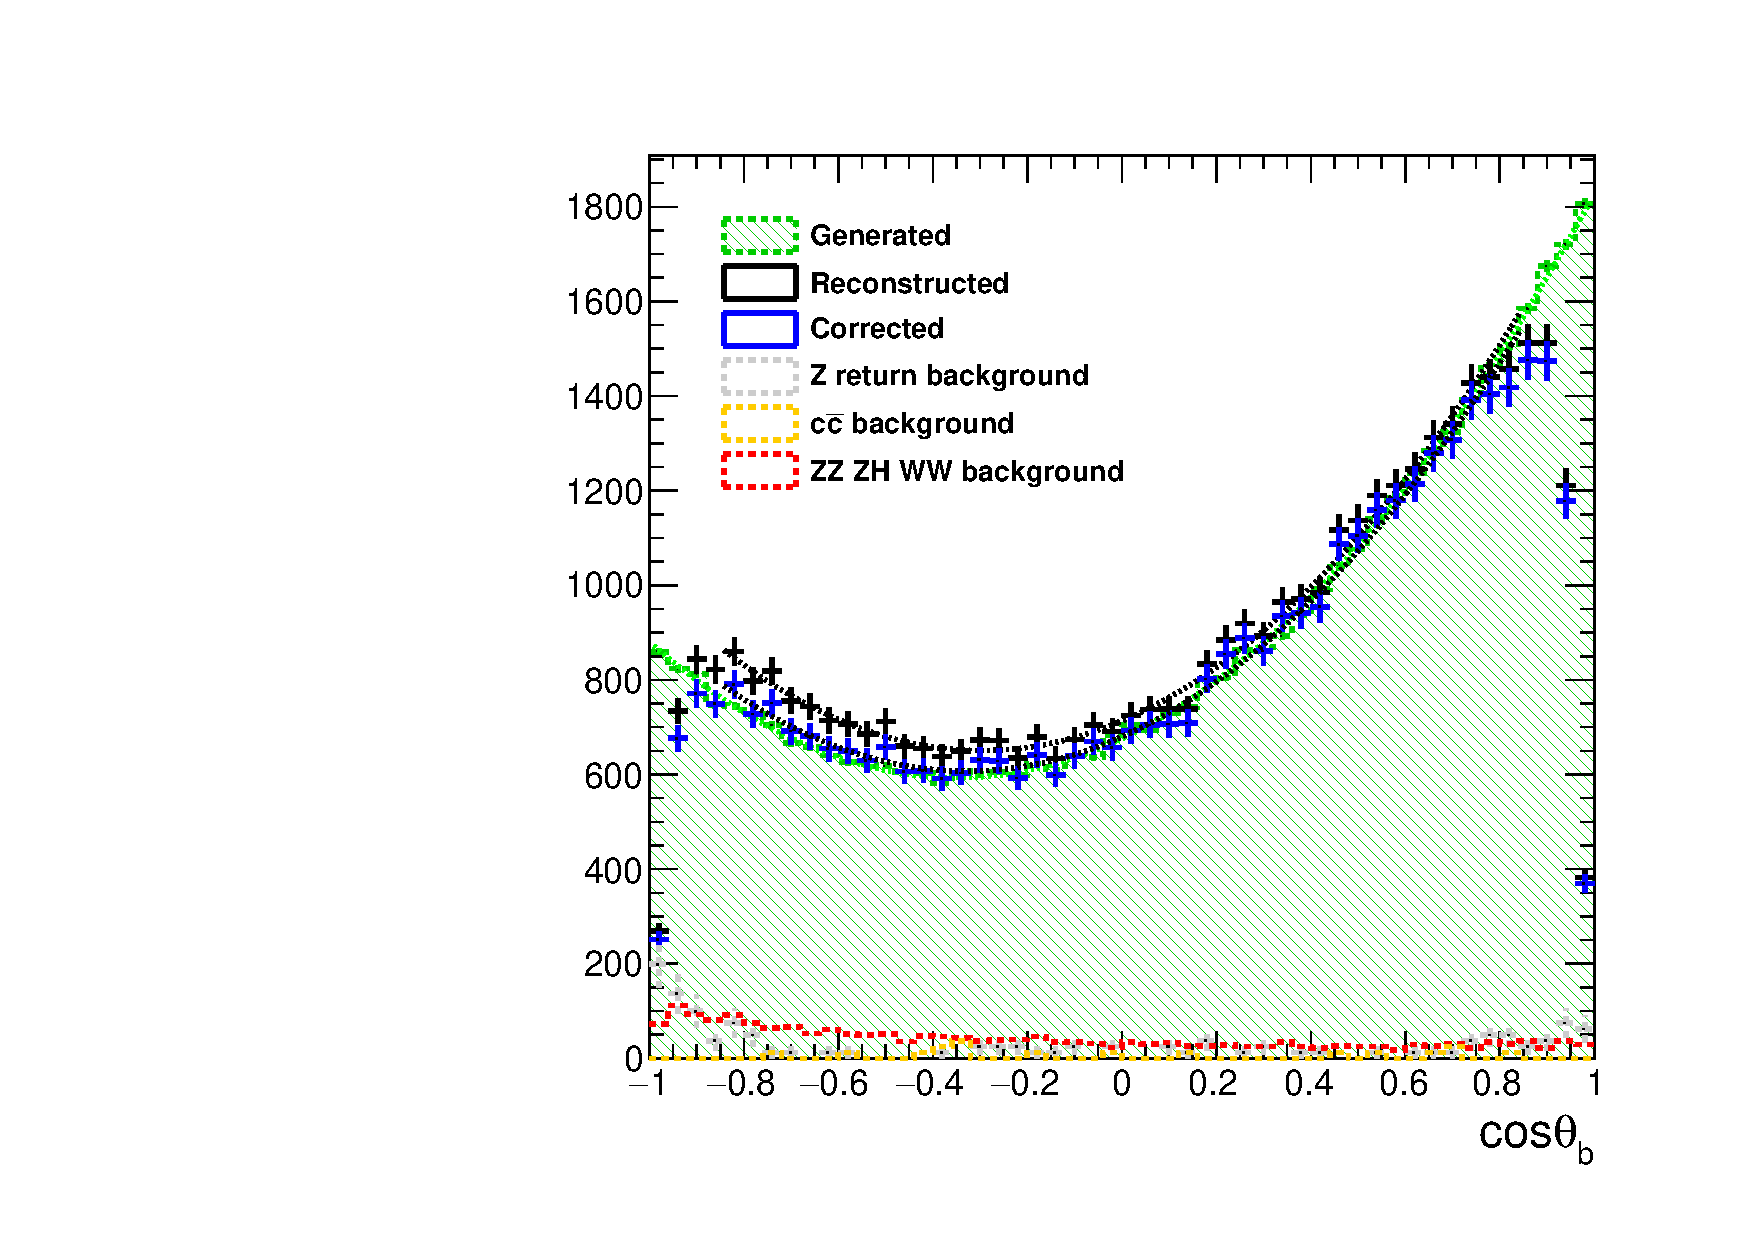
\includegraphics[width=0.45\linewidth]{./chapters/figures/basymmetry-final-right.pdf}
	\caption{Polar angle distribution $\cos{\theta_b}$ of generated $b$-quarks and final reconstructed 
         $b$-jets including any SM  background remaining after event selection. 
         Left:  $P(e^+,e^-)=(+100\%,-100\%)$ with a zoom of the region with negative 
         $\cos{\theta_b}$.
         Right: $P(e^+,e^-)=(-100\%,+100\%)$. From~\cite{Bilokin:2017lco}.  }
	\label{fig:ffbar_basym}
\end{figure*}


\begin{figure}
	\centering
	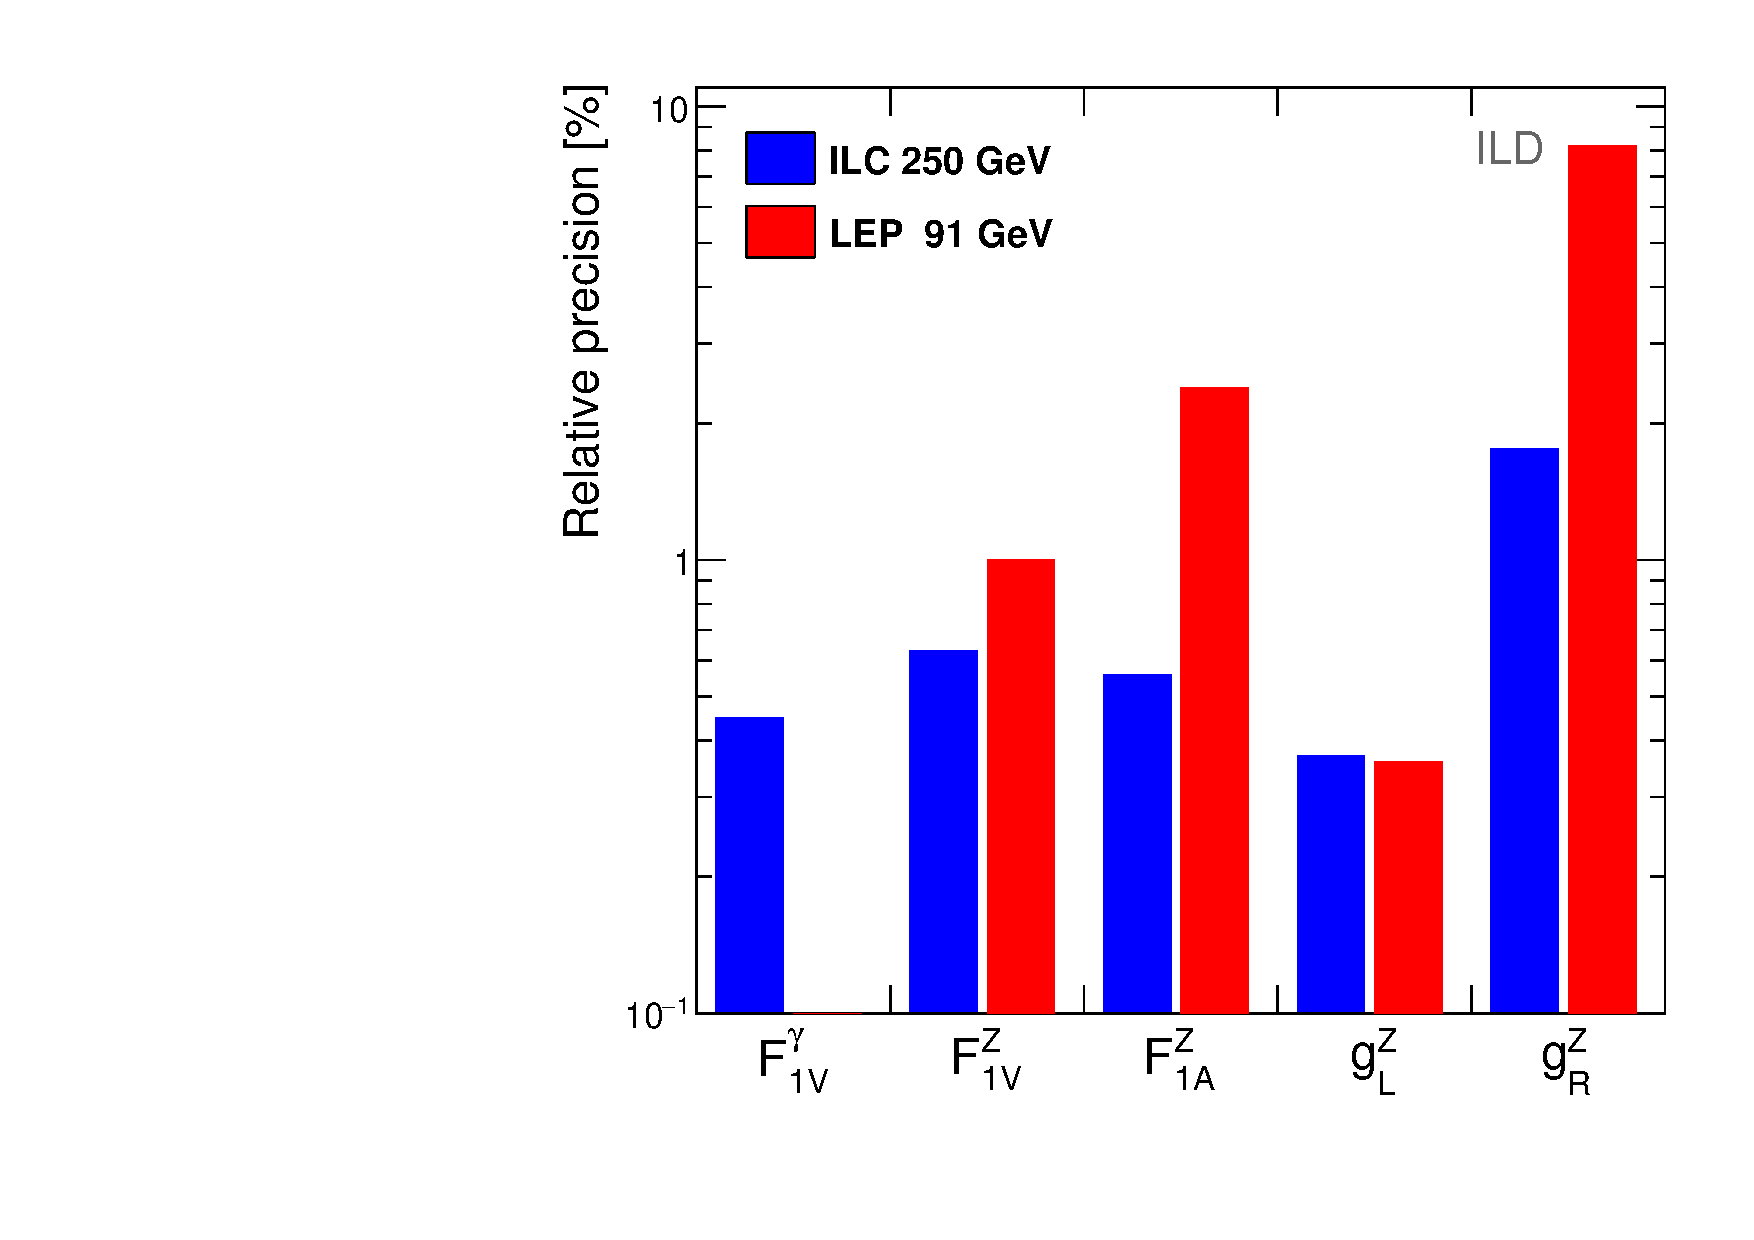
\includegraphics[width=0.95\columnwidth]{./chapters/figures/final-graph-ild.pdf}
	%	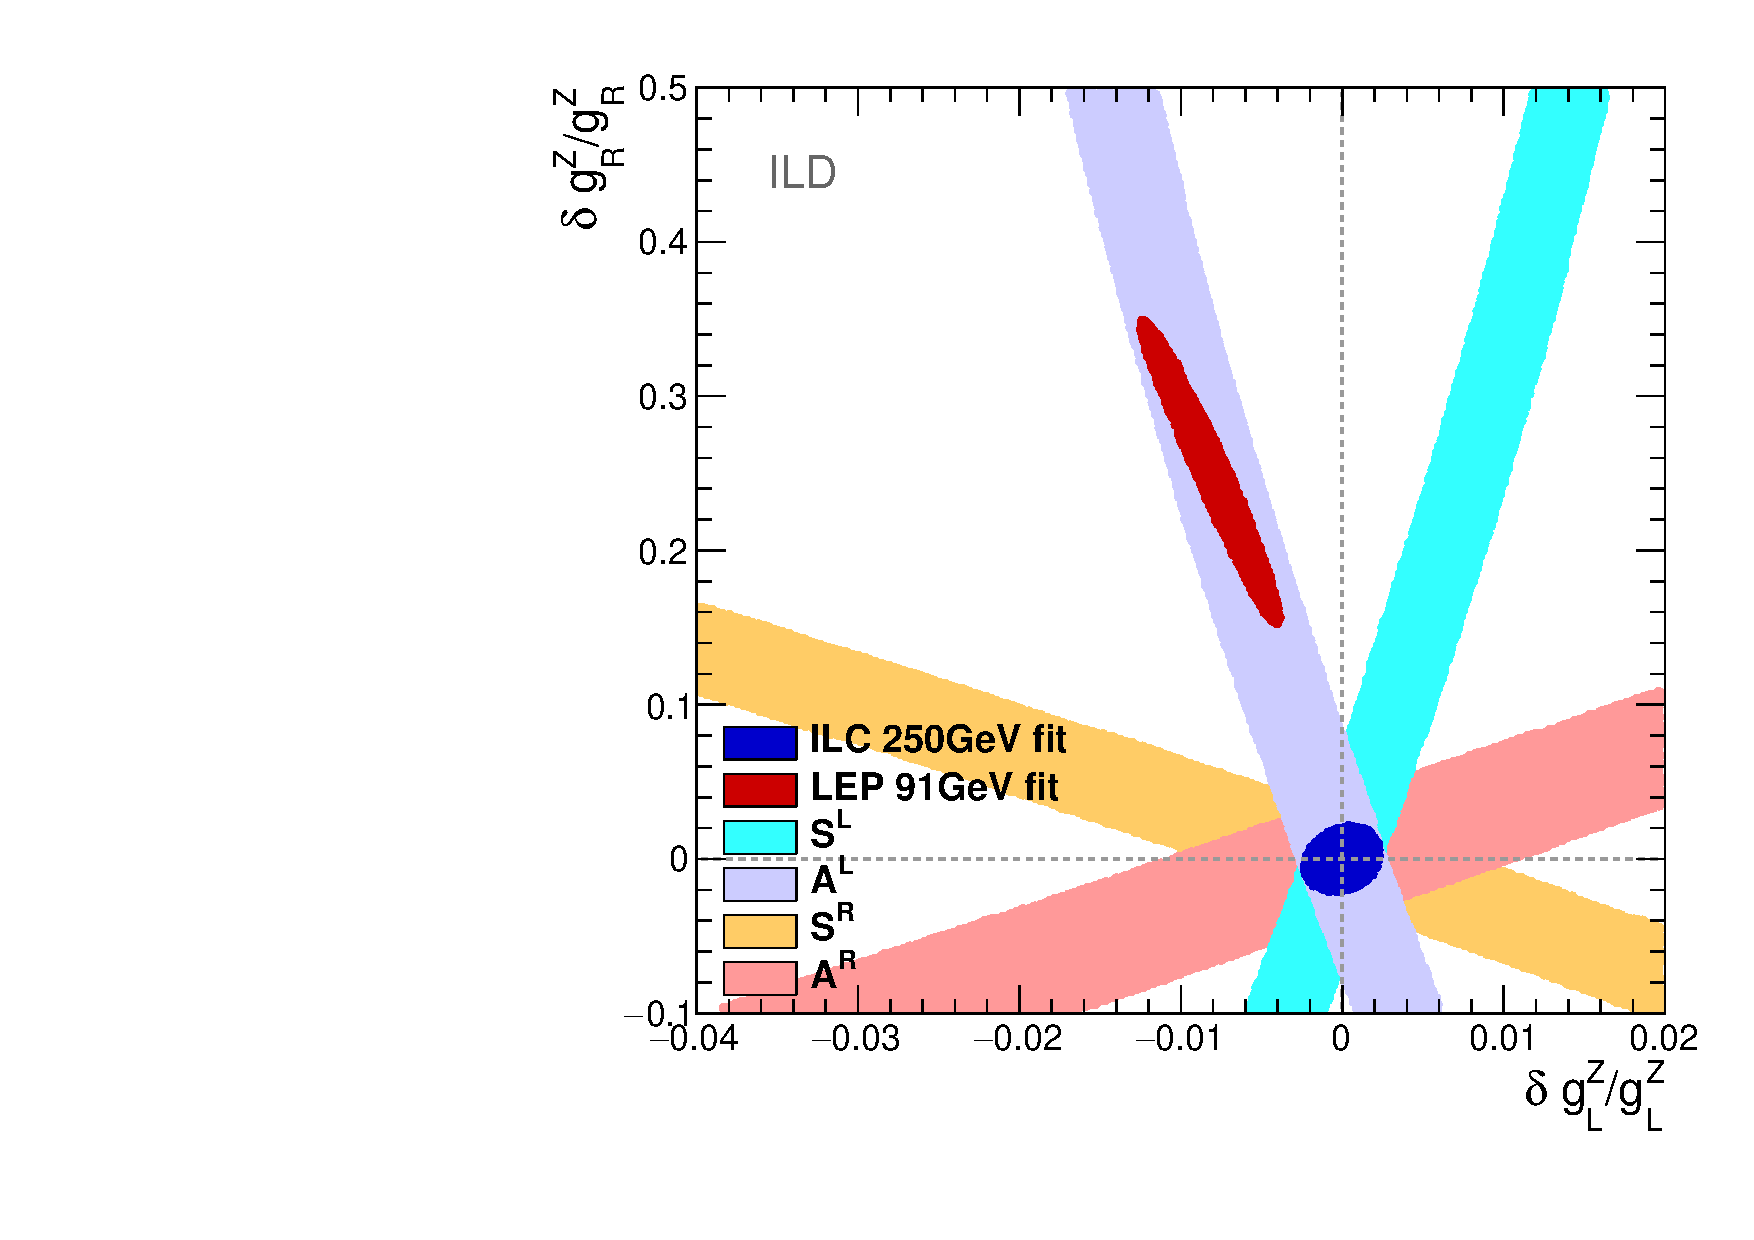
\includegraphics[width=0.95\linewidth]{./chapters/figures/ilc-precision-ild.png}
	\caption{\sl  Comparison of the LEP measurements to the expected 
                  precision at the ILC. The results of the ILC correspond to the 
                  integrated luminosity of $\mathcal{L}_I = 500$\,fb$^{-1}$ to be collected 
                   at $\sqrt{s} = 250$\,GeV before the luminosity upgrade. Final results for the
                  full 250\,GeV dataset would improve the precision further by about a factor of 2.
                   From~\cite{Bilokin:2017lco}.}
	\label{fig:LEPILCResult_3}
\end{figure}
